%% LyX 2.3.4.2 created this file.  For more info, see http://www.lyx.org/.
%% Do not edit unless you really know what you are doing.
\documentclass[11pt,spanish]{article}
\renewcommand{\rmdefault}{cmr}
\usepackage[T1]{fontenc}
\usepackage[utf8]{inputenc}
\usepackage{geometry}
\geometry{verbose,tmargin=2cm,bmargin=2cm,lmargin=2cm,rmargin=2cm}
\setlength{\parskip}{\bigskipamount}
\setlength{\parindent}{0pt}
\usepackage{amstext}
\usepackage{amsthm}
\usepackage{amssymb}
\usepackage{graphicx}

\makeatletter
%%%%%%%%%%%%%%%%%%%%%%%%%%%%%% Textclass specific LaTeX commands.
\theoremstyle{definition}
\newtheorem{example}{\protect\examplename}[section]
\theoremstyle{definition}
\newtheorem{xca}{\protect\exercisename}[section]
\theoremstyle{remark}
\newtheorem{rem}{\protect\remarkname}[section]
\theoremstyle{plain}
\newtheorem{thm}{\protect\theoremname}[section]

%%%%%%%%%%%%%%%%%%%%%%%%%%%%%% User specified LaTeX commands.
\usepackage{titling}
\setlength{\droptitle}{-2cm}
\usepackage{multicol}
\usepackage{enumitem}
\usepackage{proof}
\usepackage{mathrsfs}
\usepackage{amsfonts}
\usepackage{forest}
\usepackage{ebproof}
\usepackage{amssymb}
\definecolor{Guinda}{rgb}{0.49, 0.05, 0.12}
\definecolor{Rojo}{rgb}{0.8, 0, 0}
\definecolor{Verde}{rgb}{0,0.4,0}
\definecolor{Azul}{rgb}{0,0.4,0.4}
\definecolor{Naranja}{rgb}{0.8,0.4,0}
\usepackage{tikz}
\usetikzlibrary{automata, positioning, arrows}
\raggedcolumns

\makeatother

\usepackage{babel}
\addto\shorthandsspanish{\spanishdeactivate{~<>.}}

\usepackage{listings}
\lstset{mathescape=true}
\providecommand{\examplename}{Ejemplo}
\providecommand{\exercisename}{Ejercicio}
\providecommand{\remarkname}{Observación}
\providecommand{\theoremname}{Teorema}

\begin{document}
\title{Teoría de la Computación, 2021-1\\
Nota de clase 5: Autómatas Finitos con $\varepsilon$-transiciones\thanks{Tomada de \cite{key-1} con ligeras modificaciones.}}
\author{Manuel Soto Romero}
\date{\today \\ Colegio de Ciencia y Tecnología UACM}

\maketitle
\renewcommand*{\thefootnote}{\arabic{footnote}}
\setcounter{footnote}{0}
\setcounter{section}{5}
\renewcommand*\lstlistingname{C\'odigo}

\subsection{Definición}

Un \emph{autómata finito con $\varepsilon$-transiciones (AFN-$\varepsilon$)
}es un autómata no determinista $M=\left\langle \Sigma,Q,q_{0},F,\delta\right\rangle $
en el que la función de transición está definida como:

\[
\delta:Q\times\left(\Sigma\cup\left\{ \varepsilon\right\} \right)\rightarrow\mathcal{P}\left(Q\right)
\]

La transición $\delta\left(q,\varepsilon\right)=\left\{ p_{i1},...,p_{in}\right\} $,
llamada \emph{transición $\varepsilon$} o \emph{transición espontánea,
}tiene el siguiente significado computacional: estando en el estado
$q$, el autómata puede cambiar a uno cualquier de los estados $p_{i1},...,p_{in}$,
independientemente del símbolo leído. Dicho de otra manera, las transiciones
$\varepsilon$ permiten al autómata cambiar internamente de estado
sin consumir el símbolo leído.

En el diagrama del autómata, las transiciones $\varepsilon$ dan lugar
a aristas con etiquetas $\varepsilon$. Una cadena de entrada $w$
es aceptada por un AFN-$\varepsilon$ si existe por lo menos una trayectoria,
desde el estado $q_{0}$, cuyas etiquetas son exactamente los símbolos
de $w$, intercalados con cero, uno o más $\varepsilon$s.

En los autómatas AFN-$\varepsilon$, al igual que en los AFN, puede
haber múltiples camnios para una misma cadena de entrada. Veamos un
ejemplo:

\begin{center}
\begin{tikzpicture}[->,shorten >=1pt,auto,node distance=2cm,transform shape] 

\node[state, initial, initial text=] (0) {$q_0$}; 
\node[state, right of=0, above of=0] (1) {$q_1$};
\node[state, right of=1, accepting, accepting] (2) {$q_2$};
\node[state, right of=0, below of=0] (3) {$q_3$};
\node[state, right of=3, accepting] (4) {$q_4$};


\draw (0) edge[bend left] node{$\varepsilon$} (1)
      (0) edge[bend right] node{$a$} (3)
	  (1) edge[loop above] node{$a$} (1)
      (1) edge[bend left] node{$b$} (2)
      (2) edge[loop above] node{$b$} (2)
      (3) edge[loop below] node{$b$} (3)
      (3) edge[bend right] node{$\varepsilon$} (4)
      (4) edge[loop below] node{$a$} (4)
;

\end{tikzpicture}
\end{center}

Ejemplos de cadenas aceptadas por este autómata son:
\begin{itemize}
\item $aab$
\item $abaa$
\item $abbaa$
\end{itemize}
Los AFN-$\varepsilon$ nos dan más libertada en el diseño de autómatas,
especialmente cuando tenemos varias concatenaciones.

\bigskip{}

\begin{example}
\label{exa:.Ejemplo 1}$\Sigma=\left\{ a,b,c\right\} $. $L=a^{*}b^{*}c^{*}$

AFN que acepta a $L$:
\end{example}
\begin{center}
\begin{tikzpicture}[->,shorten >=1pt,auto,node distance=2cm,transform shape] 

\node[state, initial, initial text=,accepting] (0) {$q_0$}; 
\node[state, right of=0,accepting] (1) {$q_1$};
\node[state, right of=1, accepting] (2) {$q_2$};


\draw (0) edge[loop above] node{$a$} (0)
      (0) edge[bend left] node{$b$} (1)
      (0) edge[bend right=45] node{$c$} (2)
	  (1) edge[loop above] node{$b$} (1)
      (1) edge[bend left] node{$c$} (2)
      (2) edge[loop above] node{$c$} (2)
;

\end{tikzpicture}
\end{center}

AFN-$\varepsilon$ que acepta a $L$:

\begin{center}
\begin{tikzpicture}[->,shorten >=1pt,auto,node distance=2cm,transform shape] 

\node[state, initial, initial text=,accepting] (0) {$q_0$}; 
\node[state, right of=0,accepting] (1) {$q_1$};
\node[state, right of=1, accepting] (2) {$q_2$};


\draw (0) edge[loop above] node{$a$} (0)
      (0) edge[bend left] node{$\varepsilon$} (1)
	  (1) edge[loop above] node{$b$} (1)
      (1) edge[bend left] node{$\varepsilon$} (2)
      (2) edge[loop above] node{$c$} (2)
;

\end{tikzpicture}
\end{center}

Este autómata es muy similar a la expresión regular $a^{*}b^{*}c^{*}$:
las concatenaciones son reemplazadas por transiciones $\varepsilon$.

\bigskip{}

\begin{example}
$\Sigma=\left\{ a,b\right\} $. $L=\text{lenguaje de todas las cadenas sobre \ensuremath{\Sigma} que tienen un número par de as o un número par de bs.}$

AFD que acepta el lenguaje de las cadenas con un número par de $a$s:
\end{example}
\begin{center}
\begin{tikzpicture}[->,shorten >=1pt,auto,node distance=2cm,transform shape] 

\node[state, initial, initial text=,accepting] (0) {$q_0$}; 
\node[state, right of=0] (1) {$q_1$};


\draw (0) edge[bend left] node{$a$} (1)
      (0) edge[loop above] node{$b$} (0)
      (1) edge[bend left] node{$a$} (0)
	  (1) edge[loop above] node{$b$} (1)
;

\end{tikzpicture}
\end{center}

AFD que acepta el lenguaje de las cadenas con un número par de $b$s:

\begin{center}
\begin{tikzpicture}[->,shorten >=1pt,auto,node distance=2cm,transform shape] 

\node[state, initial, initial text=,accepting] (0) {$q_0$}; 
\node[state, right of=0] (1) {$q_1$};


\draw (0) edge[bend left] node{$b$} (1)
      (0) edge[loop above] node{$a$} (0)
      (1) edge[bend left] node{$b$} (0)
	  (1) edge[loop above] node{$a$} (1)
;

\end{tikzpicture}
\end{center}

AFN-$\varepsilon$ que acepta el lenguaje de las cadenas con un número
par de $a$s o número par de $b$s:

\begin{center}
\begin{tikzpicture}[->,shorten >=1pt,auto,node distance=2cm,transform shape] 

\node[state, initial, initial text=,accepting] (0) {$q_0$}; 
\node[state, right of=0, above of=0,accepting] (1) {$q_1$};
\node[state, right of=1,] (2) {$q_2$};
\node[state, right of=0, below of=0,accepting] (3) {$q_3$};
\node[state, right of=3] (4) {$q_4$};


\draw (0) edge[bend left] node{$\varepsilon$} (1)
      (0) edge[bend right] node{$\varepsilon$} (3)
	  (1) edge[loop above] node{$b$} (1)
      (1) edge[bend left] node{$a$} (2)
      (2) edge[loop above] node{$b$} (2)
      (2) edge[bend left] node{$a$} (1)
      (3) edge[loop above] node{$a$} (3)
      (3) edge[bend left] node{$b$} (4)
      (4) edge[loop above] node{$a$} (4)
      (4) edge[bend left] node{$b$} (3)
;

\end{tikzpicture}
\end{center}

A diferencia de los AFD y los AFN, en los AFN-$\varepsilon$ pueden
existir cómputos infinitos, es decir, cómputos que nunca terminan.
Esto puede suceder si el autómata ingresa a un estado desde el cual
haya varias transiciones $\varepsilon$ encadenadas que regresen al
mismo estado. Por ejemplo, el siguiente autómata: 

\begin{center}
\begin{tikzpicture}[->,shorten >=1pt,auto,node distance=2cm,transform shape] 

\node[state] (0) {$$}; 
\node[state, right of=0] (1) {$$};
\node[state, right of=1] (2) {$$};


\draw (0) edge[bend left] node{$\varepsilon$} (1)
      (1) edge[bend left] node{$\varepsilon$} (2)
	  (2) edge[bend left] node{$\varepsilon$} (0)
;

\end{tikzpicture}
\end{center}

\bigskip{}

\begin{xca}
Diseñar un AFN-$\text{\ensuremath{\varepsilon}}$ que acepte el lenguaje
$\left(ab+b\right)^{*}ab^{*}$, sobre $\Sigma=\left\{ a,b\right\} $.
\end{xca}
%

\subsection{Equivalencia entre AFN-$\varepsilon$ y AFN}

En esta sección mostraremos que el modelo AFN-$\varepsilon$ es computacionalmente
equivalente al modelo AFN. Es decir, se pueden quitar las transiciones
$\varepsilon$ y añadir nuevas que las simulen sin alterar el lenguaje
aceptado. Comencemos con la siguiente observación.

\bigskip{}

\begin{rem}
Un AFN puede ser visto como un AFN-$\varepsilon$ en el que, simplemente
hay \emph{cero} transiciones $\varepsilon$. 
\end{rem}
%
Con esta observación, tenemos el siguiente teorema:

\bigskip{}

\begin{thm}
Dado un AFN-$\varepsilon$ $M$, se puede construir un AFN $M'$ equivalente
a $M$ tal que $L\left(M\right)=L\left(M'\right)$.
\end{thm}
%
La demostración del teorema queda fuera de los alcances de este curso,
por lo que en su lugar, presentaremos un método de tranformación.
Necesitamos primero que nada definir el concepto de \emph{$\varepsilon$-cerradura}. 

Para un estado $q$, la $\varepsilon$, denotada $ECLOSURE\left(q\right)$
es el conjunto de estados de un AFN-$\varepsilon$ a los que se puede
llegar desde $q$ por 0, 1 o más transiciones $\varepsilon$. Nótar
además que $ECLOSURE\left(q\right)\neq\delta\left(q,\varepsilon\right).$
Por definición $q\in ECLOSURE\left(q\right)$. De esta forma, la $\varepsilon$-cerradura
de un conjunto de estados $\left\{ q_{1},...,q_{k}\right\} $ se define
por:

\[
ECLOSURE\left(\left\{ q_{1},...,q_{k}\right\} \right)=ECLOSURE\left(q_{1}\right)\cup...\cup ECLOSURE\left(q_{k}\right)
\]

Además, $ECLOSURE\left(\varnothing\right)=\varnothing.$ 

De esta manera, podemos construir un AFN $M'=\left\langle \Sigma,Q,q_{0},F',\delta'\right\rangle $
a partir del AFN-$\varepsilon$ $M=\left\langle \Sigma,Q,q_{0},F,\delta\right\rangle $,
mediante la siguiente función de transición:

\[
\begin{array}{rcl}
\delta':Q\times\Sigma & \rightarrow & \mathcal{P}\left(Q\right)\\
\left(q,a\right) & \rightarrow & \delta'\left(q,a\right)=ECLOSURE\left(\delta\left(ECLOSURE\left(q\right),a\right)\right)
\end{array}
\]

$M'$ simula así las transiciones $\varepsilon$ de $M$ teniendo
en cuenta todas las posibles trayectorias. $F'$ se define como:

\[
F'=\left\{ q\in Q:ECLOSURE\left(q\right)\text{ contiene al menos un estado de aceptación}\right\} 
\]

Es decir, los estados de aceptación de $M'$ incluyen los estados
de aceptación de $M$ y aquellos estados desde los cuales se puede
llegar a un estado de aceptación por medio de una o más transiciones
$\varepsilon$.

Veamos un ejemplo.

\bigskip{}

\begin{example}
Vamos a ilustrar el método anterior con el autómata del Ejemplo \ref{exa:.Ejemplo 1}
al que llamaremos $M$:
\end{example}
\begin{center}
\begin{tikzpicture}[->,shorten >=1pt,auto,node distance=2cm,transform shape] 

\node[state, initial, initial text=,accepting] (0) {$q_0$}; 
\node[state, right of=0,accepting] (1) {$q_1$};
\node[state, right of=1, accepting] (2) {$q_2$};


\draw (0) edge[loop above] node{$a$} (0)
      (0) edge[bend left] node{$\varepsilon$} (1)
	  (1) edge[loop above] node{$b$} (1)
      (1) edge[bend left] node{$\varepsilon$} (2)
      (2) edge[loop above] node{$c$} (2)
;

\end{tikzpicture}
\end{center}

Recordemos que $L$$\left(M\right)=a^{*}b^{*}c^{*}$. Comencemos entonces
calculando la $\varepsilon$ cerradura de cada estado de nuestro autómata.

\[
\begin{array}{lcl}
ECLOSURE\left(q_{0}\right) & = & \left\{ q_{0},q_{1},q_{2}\right\} \\
ECLOSURE\left(q_{1}\right) & = & \left\{ q_{1},q_{2}\right\} \\
ECLOSURE\left(q_{2}\right) & = & \left\{ q_{2}\right\} 
\end{array}
\]

A partir de aquí construimos las transiciones correspondientes, abreviamos
\emph{ECLOSURE como EC}:

\[
\begin{array}{lcl}
\delta'\left(q_{0},a\right) & = & EC\left(\delta\left(EC\left(q_{0}\right),a\right)\right)=EC\left(\delta\left(\left\{ q_{0},q_{1},q_{2}\right\} ,a\right)\right)=EC\left(\left\{ q_{0}\right\} \right)=\left\{ q_{0},q_{1},q_{2}\right\} \\
\delta'\left(q_{0},b\right) & = & EC\left(\delta\left(EC\left(q_{0}\right),b\right)\right)=EC\left(\delta\left(\left\{ q_{0},q_{1},q_{2}\right\} ,b\right)\right)=EC\left(\left\{ q_{1}\right\} \right)=\left\{ q_{1},q_{2}\right\} \\
\delta'\left(q_{0},c\right) & = & EC\left(\delta\left(EC\left(q_{0}\right),c\right)\right)=EC\left(\delta\left(\left\{ q_{0},q_{1},q_{2}\right\} ,c\right)\right)=EC\left(\left\{ q_{2}\right\} \right)=\left\{ q_{2}\right\} \\
\delta'\left(q_{1},a\right) & = & EC\left(\delta\left(EC\left(q_{1}\right),a\right)\right)=EC\left(\delta\left(\left\{ q_{1},q_{2}\right\} ,a\right)\right)=EC\left(\varnothing\right)=\varnothing\\
\delta'\left(q_{1},b\right) & = & EC\left(\delta\left(EC\left(q_{1}\right),b\right)\right)=EC\left(\delta\left(\left\{ q_{1},q_{2}\right\} ,b\right)\right)=EC\left(\left\{ q_{1}\right\} \right)=\left\{ q_{1},q_{2}\right\} \\
\delta'\left(q_{1},c\right) & = & EC\left(\delta\left(EC\left(q_{1}\right),c\right)\right)=EC\left(\delta\left(\left\{ q_{1},q_{2}\right\} ,c\right)\right)=EC\left(\left\{ q_{2}\right\} \right)=\left\{ q_{2}\right\} \\
\delta\left(q_{2},a\right) & = & EC\left(\delta\left(EC\left(q_{2}\right),a\right)\right)=EC\left(\delta\left(\left\{ q_{2}\right\} ,a\right)\right)=EC\left(\varnothing\right)=\varnothing\\
\delta\left(q_{2},b\right) & = & EC\left(\delta\left(EC\left(q_{2}\right),b\right)\right)=EC\left(\delta\left(\left\{ q_{2}\right\} ,b\right)\right)=EC\left(\varnothing\right)=\varnothing\\
\delta\left(q_{2},c\right) & = & EC\left(\delta\left(EC\left(q_{2}\right),c\right)\right)=EC\left(\delta\left(\left\{ q_{2}\right\} ,c\right)\right)=EC\left(\left\{ q_{2}\right\} \right)=\left\{ q_{2}\right\} 
\end{array}
\]

El conjunto de estados finales es $\left\{ q_{0,}q_{1},q_{2}\right\} $
dado que las cerraduras de todos los estados contienen estados finales.
De esta forma, el autómata AFN queda como:

\begin{center}
\begin{tikzpicture}[->,shorten >=1pt,auto,node distance=2cm,transform shape] 

\node[state, initial, initial text=,accepting] (0) {$q_0$}; 
\node[state, right of=0,accepting] (1) {$q_1$};
\node[state, right of=1, accepting] (2) {$q_2$};


\draw (0) edge[loop above] node{$a$} (0)
      (0) edge[] node{$a,b$} (1)
	  (0) edge[bend left=50] node{$a,b,c$} (2)
	  (1) edge[loop below] node{$b$} (1)
      (1) edge[] node{$b,c$} (2)
      (2) edge[loop above] node{$c$} (2)
;

\end{tikzpicture}
\end{center}

\bigskip{}

\begin{xca}
Construye un AFN equivalente al siguiente AFN-$\varepsilon$:
\end{xca}
\begin{center}
\begin{tikzpicture}[->,shorten >=1pt,auto,node distance=3cm,transform shape] 

\node[state, initial, initial text=,accepting] (0) {$q_0$}; 
\node[state, right of=0] (1) {$q_1$};
\node[state, below of=0] (2) {$q_2$};
\node[state, right of=2] (3) {$q_3$};


\draw (0) edge[bend left] node{$\varepsilon$} (1)
      (0) edge[] node{$a,\varepsilon$} (2)
	  (1) edge[bend left] node{$b$} (0)
      (2) edge[] node{$\varepsilon$} (3)
      (3) edge[] node{$b$} (0)
;

\end{tikzpicture}
\end{center}


\subsection{Teorema de Kleene}

En las notas y secciones anteriores, se ha mostrado la equivalencia
computacional entre los AFD, AFN y AFN-$\varepsilon$, lo cual puede
ser descrito de la siguiente forma:

\[
\text{AFD}\equiv\text{AFN}\equiv\text{AFN-}\varepsilon
\]

Esto quiere decir que para cada uno de estos tipos de autómatas se
pueden construir otro tipo de autómatas equivalentes. Por lo tanto,
estos tres modelos aceptan exactamente los mismos modelos. El Teorema
de Kleene establece que tales lenguajes son precisamente los lenguajes
regulares.

\bigskip{}

\begin{thm}
Un lenguaje es regular si y sólo si es aceptado por un autómata finito
(AFD o AFN o AFN-$\varepsilon$).
\end{thm}
%
La demostración de este teorema queda fuera de los alcances del curso.
Sin embargo, la misma demostración nos permite analizar la equivalencia
que hay entre las expresiones regulares y los autómatas finitos (en
ambos sentidos) por medio de dos partes: La Parte I demuestra que
dada una expresión regular $R$ sobre un alfabeto $\Sigma$, se puede
construir un AFN-$\varepsilon$ $M$ tal que el lenguaje aceptado
por $M$ sea exactamente el lenguaje representado por $R$. Por otro
lado, la Parte II demuestra que para todo $AFN$ $M$ existe una expresión
regular $R$ tal que $L(M)=R$. Para los fines de este curso nos enfocaremos
en la Parte I de la demostración desde un enfoque algorítmico.

Recordemos que una expresión regular se define recursivamente como:

Sea $\Sigma$ un alfabeto. La \emph{expresión regular} sobre $\Sigma$
y los conjuntos que ellas denotan son definidos recursivamente como
sigue:
\begin{itemize}
\item $\varnothing$ es una expresión regular y denota el conjunto vacío.
\item $\varepsilon$ es una expresión regular y denota el conjunto $\left\{ \varepsilon\right\} $.
\item Para cada $a$ en $\Sigma$, $a$ es una expresión regular y denota
el conjunto $\left\{ a\right\} $.
\item Si $r$ y $s$ son expresiones regulares denotando el lenguaje $R$
y $S$ respectivamente entonces $\left(r+s\right),rs,r^{*}$ son expresiones
regulares que denotan los conjuntos $R\cup S,RS$ y $R^{*}$, respectivamente.
\end{itemize}
De esta forma, a partir de cada una de las construcciones anteriores,
podemos construir también autómatas que acepten los lenguajes que
representan cada una de éstas. Veamos cada uno de estos casos. Es
importante notar que el autómata obtenido será un AFN-$\varepsilon$.

\bigskip{}

\begin{multicols}{2}

\textbf{Caso 1 ($\varnothing$)}

El siguiente autómata acepta el lenguaje $\varnothing$, es decir
el lenguaje representado por la expresión regular $R=\varnothing$.

\columnbreak

\emph{Autómata}
\begin{center}
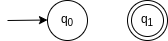
\includegraphics[scale=0.6]{imagenes/automata1}
\par\end{center}

\end{multicols}

\bigskip{}

\begin{multicols}{2}

\textbf{Caso 2 ($\varepsilon$)}

El siguiente autómata acepta el lenguaje $\left\{ \varepsilon\right\} $,
es decir, el lenguaje representado por la expresión regular $R=\varepsilon$.

\columnbreak

\emph{Autómata}
\begin{center}
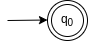
\includegraphics[scale=0.6]{imagenes/automata2}
\par\end{center}

\end{multicols}

\bigskip{}

\begin{multicols}{2}

\textbf{Caso 3 ($a$)}

El siguiente autómata acepta el lenguaje $\left\{ a\right\} $, $a\in\Sigma$,
es decir, el lenguaje representado por la expresión regular $R=a$.

\columnbreak

\emph{Autómata}
\begin{center}
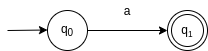
\includegraphics[scale=0.6]{imagenes/automata3}
\par\end{center}

\end{multicols}

Para los siguientes casos, supóngase que para las expresiones regulares
$R$ y $S$ existen AFN-$\varepsilon$ $M_{1}$ y $M_{2}$ tales que
$L\left(M_{1}\right)=L\left(R\right)$ y $L\left(M_{2}\right)=S$.
Esquemáticamente vamos a presentar los autómatas $M_{1}$ y $M_{2}$
de la siguiente forma:
\begin{center}
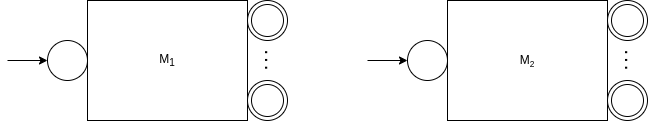
\includegraphics[scale=0.6]{imagenes/automata4}
\par\end{center}

\bigskip{}

\begin{multicols}{2}

\textbf{Caso 4 ($R+S$)}

Los autómatas $M_{1}$ y $M_{2}$ se conectan en paralelo y los estados
finales del nuevo autómata son los estados de $M_{1}$ junto con los
de $M_{2}$.

\columnbreak

\emph{Autómata}
\begin{center}
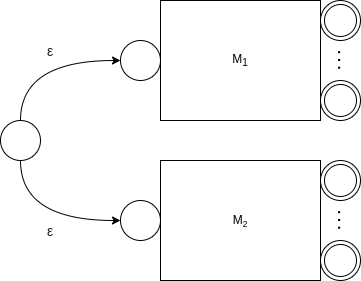
\includegraphics[scale=0.5]{imagenes/automata5}
\par\end{center}

\end{multicols}

\bigskip{}

\begin{multicols}{2}

\textbf{Caso 5 ($RS$)}

Los autómatas $M_{1}$ y $M_{2}$ se conectan en serie y los estados
finales del nuevo autómata son únicamente los estados finales de $M_{2}$.

\columnbreak

\emph{Autómata}
\begin{center}
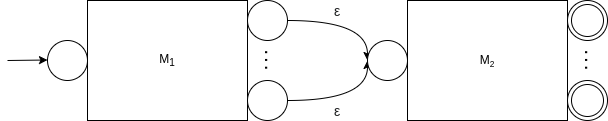
\includegraphics[scale=0.4]{imagenes/automata6}
\par\end{center}

\end{multicols}

\bigskip{}

\begin{multicols}{2}

\textbf{Caso 6 ($R^{*}$)}

Los estados finales del nuevo autómata son los estados finales de
$M_{1}$ junto con el estado inicial.

\columnbreak

\emph{Autómata}
\begin{center}
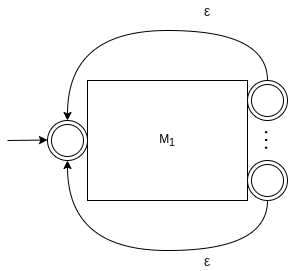
\includegraphics[scale=0.5]{imagenes/automata7}
\par\end{center}

\end{multicols}

\subsubsection{Ejemplo}

De acuerdo con las construcciones presentadas, a continuación veremos
algunos ejemplos, sin embargo antes de empezar, analicemos el siguiente
autómata que acepta el lenguaje $a^{*}$:

\begin{center}
\begin{tikzpicture}[->,shorten >=1pt,auto,node distance=3cm,transform shape] 

\node[state, initial, initial text=,accepting] (0) {$$}; 
\node[state, right of=0,accepting] (1) {$$};


\draw (0) edge[] node{$a$} (1)
      (1) edge[bend right=60] node{$\varepsilon$} (0)
;

\end{tikzpicture}
\end{center}

Para simplificar las próximas construcciones, usaremos en su lugar
el ciclo de un estado:

\begin{center}
\begin{tikzpicture}[->,shorten >=1pt,auto,node distance=3cm,transform shape] 

\node[state, initial, initial text=,accepting] (0) {$$}; 


\draw (0) edge[loop above] node{$a$} (0)
;

\end{tikzpicture}
\end{center}

\bigskip{}

\begin{example}
Vamos a utilizar el procedimiento anterior para construir un AFN-$\varepsilon$
que acepte el lenguaje $a^{*}\left(ab+ba\right)^{*}+a\left(b+a^{*}\right)$
sobre el alfabeto $\left\{ a,b\right\} $.
\end{example}
\begin{itemize}
\item Autómata que acepta $ab$:

\begin{center}
\begin{tikzpicture}[->,shorten >=1pt,auto,node distance=2cm,transform shape] 

\node[state, initial, initial text=] (0) {$$};
\node[state, right of=0] (1) {$$};
\node[state, right of=1] (2) {$$};
\node[state, right of=2, accepting] (3) {$$};


\draw (0) edge[] node{$a$} (1)
      (1) edge[] node{$\varepsilon$} (2)
      (2) edge[] node{$b$} (3)
;

\end{tikzpicture}
\end{center}
\item Autómata que acepta $ba$:

\begin{center}
\begin{tikzpicture}[->,shorten >=1pt,auto,node distance=2cm,transform shape] 

\node[state, initial, initial text=] (0) {$$};
\node[state, right of=0] (1) {$$};
\node[state, right of=1] (2) {$$};
\node[state, right of=2, accepting] (3) {$$};


\draw (0) edge[] node{$b$} (1)
      (1) edge[] node{$\varepsilon$} (2)
      (2) edge[] node{$a$} (3)
;

\end{tikzpicture}
\end{center}
\item Autómata que acepta $ab+ba$:

\begin{center}
\begin{tikzpicture}[->,shorten >=1pt,auto,node distance=2cm,transform shape] 

\node[state, initial, initial text=] (0) {$$};
\node[state, right of=0,above of=0] (1) {$$};
\node[state, right of=1] (2) {$$};
\node[state, right of=2] (3) {$$};
\node[state, right of=3, accepting] (4) {$$};
\node[state, right of=0,below of=0] (5) {$$};
\node[state, right of=5] (6) {$$};
\node[state, right of=6] (7) {$$};
\node[state, right of=7, accepting] (8) {$$};


\draw (0) edge[bend left] node{$\varepsilon$} (1)
	  (0) edge[bend right] node{$\varepsilon$} (5)
      (1) edge[] node{$a$} (2)
      (2) edge[] node{$\varepsilon$} (3)
      (3) edge[] node{$b$} (4)
	  (5) edge[] node{$b$} (6)
      (6) edge[] node{$\varepsilon$} (7)
      (7) edge[] node{$a$} (8)
;

\end{tikzpicture}
\end{center}
\item Autómata que acepta $\left(ab+ba\right)$$^{*}$:

\begin{center}
\begin{tikzpicture}[->,shorten >=1pt,auto,node distance=2cm,transform shape] 

\node[state, initial, initial text=,accepting] (0) {$$};
\node[state, right of=0,above of=0] (1) {$$};
\node[state, right of=1] (2) {$$};
\node[state, right of=2] (3) {$$};
\node[state, right of=3, accepting] (4) {$$};
\node[state, right of=0,below of=0] (5) {$$};
\node[state, right of=5] (6) {$$};
\node[state, right of=6] (7) {$$};
\node[state, right of=7, accepting] (8) {$$};


\draw (0) edge[bend left] node{$\varepsilon$} (1)
	  (0) edge[bend right] node{$\varepsilon$} (5)
      (1) edge[] node{$a$} (2)
      (2) edge[] node{$\varepsilon$} (3)
      (3) edge[] node{$b$} (4)
      (4) edge[bend right=80] node{$\varepsilon$} (0)
	  (5) edge[] node{$b$} (6)
      (6) edge[] node{$\varepsilon$} (7)
      (7) edge[] node{$a$} (8)
      (8) edge[bend left=80] node{$\varepsilon$} (0)
;

\end{tikzpicture}
\end{center}
\item Autómata que acepta $a^{*}\left(ab+ba\right)$$^{*}$:

\begin{center}
\begin{tikzpicture}[->,shorten >=1pt,auto,node distance=2cm,transform shape] 

\node[state,accepting] (0) {$$};
\node[state, right of=0,above of=0] (1) {$$};
\node[state, right of=1] (2) {$$};
\node[state, right of=2] (3) {$$};
\node[state, right of=3, accepting] (4) {$$};
\node[state, right of=0,below of=0] (5) {$$};
\node[state, right of=5] (6) {$$};
\node[state, right of=6] (7) {$$};
\node[state, right of=7, accepting] (8) {$$};
\node[state, left of=0,initial,initial text=] (9) {$$};


\draw (0) edge[bend left] node{$\varepsilon$} (1)
	  (0) edge[bend right] node{$\varepsilon$} (5)
      (1) edge[] node{$a$} (2)
      (2) edge[] node{$\varepsilon$} (3)
      (3) edge[] node{$b$} (4)
      (4) edge[bend right=80] node{$\varepsilon$} (0)
	  (5) edge[] node{$b$} (6)
      (6) edge[] node{$\varepsilon$} (7)
      (7) edge[] node{$a$} (8)
      (8) edge[bend left=80] node{$\varepsilon$} (0)
      (9) edge[loop above] node{$a$} (9)
      (9) edge[] node{$\varepsilon$} (0)
;

\end{tikzpicture}
\end{center}
\item Autómata que acepta $b+a^{*}:$

\begin{center}
\begin{tikzpicture}[->,shorten >=1pt,auto,node distance=2cm,transform shape] 

\node[state, initial, initial text=] (0) {$$};
\node[state, right of=0,above of=0] (1) {$$};
\node[state, right of=0,below of=0,accepting] (2) {$$};
\node[state, right of=1, accepting] (3) {$$};


\draw (0) edge[bend left] node{$\varepsilon$} (1)
      (0) edge[bend right] node{$\varepsilon$} (2)
      (1) edge[] node{$b$} (3)
      (2) edge[loop below] node{$a$} (2)
;

\end{tikzpicture}
\end{center}
\item Autómata que acepta $a\left(b+a^{*}\right):$

\begin{center}
\begin{tikzpicture}[->,shorten >=1pt,auto,node distance=2cm,transform shape] 

\node[state] (0) {$$};
\node[state, right of=0,above of=0] (1) {$$};
\node[state, right of=0,below of=0,accepting] (2) {$$};
\node[state, right of=1, accepting] (3) {$$};
\node[state, left of=0] (4) {$$};
\node[state, left of=4,initial,initial text=] (5) {$$};

\draw (0) edge[bend left] node{$\varepsilon$} (1)
      (0) edge[bend right] node{$\varepsilon$} (2)
      (1) edge[] node{$b$} (3)
      (2) edge[loop below] node{$a$} (2)
      (5) edge[] node{$a$} (4)
      (4) edge[] node{$\varepsilon$} (0)
;

\end{tikzpicture}
\end{center}
\item Autómata que acepta $a^{*}\left(ab+ba\right)^{*}+a\left(b+a^{*}\right)$:

\begin{center}
\begin{tikzpicture}[->,shorten >=1pt,auto,node distance=2cm,transform shape] 

\node[state,left of=9,below of=9,initial,initial text=] (16) {$$};

\node[state,accepting] (0) {$$};
\node[state, right of=0,above of=0] (1) {$$};
\node[state, right of=1] (2) {$$};
\node[state, right of=2] (3) {$$};
\node[state, right of=3, accepting] (4) {$$};
\node[state, right of=0,below of=0] (5) {$$};
\node[state, right of=5] (6) {$$};
\node[state, right of=6] (7) {$$};
\node[state, right of=7, accepting] (8) {$$};
\node[state, left of=0] (9) {$$};
\node[state, below=5cm of 16,right of=16] (10) {$$};
\node[state, right of=10] (11) {$$};
\node[state, right of=11] (12) {$$};
\node[state, right of=12, above of=12] (13) {$$};
\node[state, right of=13, accepting] (14) {$$};
\node[state, right of=12, below of=12,accepting] (15) {$$};




\draw (0) edge[bend left] node{$\varepsilon$} (1)
	  (0) edge[bend right] node{$\varepsilon$} (5)
      (1) edge[] node{$a$} (2)
      (2) edge[] node{$\varepsilon$} (3)
      (3) edge[] node{$b$} (4)
      (4) edge[bend right=80] node{$\varepsilon$} (0)
	  (5) edge[] node{$b$} (6)
      (6) edge[] node{$\varepsilon$} (7)
      (7) edge[] node{$a$} (8)
      (8) edge[bend left=80] node{$\varepsilon$} (0)
      (9) edge[loop above] node{$a$} (9)
      (9) edge[] node{$\varepsilon$} (0)

      (16) edge[bend left] node{$\varepsilon$} (9)
	  (16) edge[bend right] node{$\varepsilon$} (10)

      (10) edge[] node{$a$} (11)
      (11) edge[] node{$\varepsilon$} (12)
      (12) edge[bend left] node{$\varepsilon$} (13)
      (13) edge[] node{$b$} (14)
      (12) edge[bend right] node{$\varepsilon$} (15)
      (15) edge[loop below] node{$a$} (15)
     
;

\end{tikzpicture}
\end{center}
\end{itemize}
\bigskip{}

\begin{xca}
Diseñar autómatas AFN-$\varepsilon$ que acepten los siguientes lenguajes
sobre el alfabeto $\Sigma=\left\{ a,b,c\right\} $:
\end{xca}
\begin{itemize}
\item $a^{*}\left(b+ab^{*}+ab^{*}a\right)c^{*}+\left(a+b\right)\left(a+ac\right)^{*}$
\item $c^{*}a\left(a+ba\right)^{*}\left(abc\right)^{*}+c^{*}\left(a+cb^{*}c\right)$
\end{itemize}
\begin{thebibliography}{1}
\bibitem{key-1}Rodrigo De Castro, \emph{Notas de Clase de Teoría
de la Computación: Lenguajes, autómatas, gramáticas,} Universidad
Nacional de Colombia, Facultas de Ciencias, 2004.
\end{thebibliography}

\end{document}
